\documentclass[xcolor=table,9pt]{beamer}
\usepackage{hyperref}
\hypersetup{pdftoolbar=false,pdfwindowui=false,bookmarks=false}
\usepackage{fontspec}
\setmainfont{DejaVu Serif}
\setsansfont{DejaVu Sans}
\setmonofont{DejaVu Sans Mono}

\usepackage{amssymb,amsfonts,amsmath,mathtext}
\usepackage{cite,enumerate,float,indentfirst}
\usepackage{ragged2e}
\usepackage{comment}
\usepackage{epigraph}
\usepackage{graphicx}
\usepackage{hyperref}
\usepackage{xcolor}
\usepackage{wrapfig}
\usepackage{subfig}
\usepackage{derivative}
\usepackage{setspace}
\usepackage{pgfplots}
\usepackage[absolute,overlay]{textpos}
\usepackage{media9}
\usepackage{animate}
\usepackage{multirow}
\usepackage{booktabs}
\usepackage{fontawesome}

% Настройки из style_example.tex
\captionsetup[figure]{name=\large{Рис.}}
\captionsetup[table]{name=\large{Таблица}}
\setbeamertemplate{caption}{\insertcaption}
\setbeamertemplate{caption}[numbered]
\setbeamertemplate{page number in head/foot}[totalframenumber]

% Применяем тему и цветовую схему из style_example.tex
\usetheme{Copenhagen}
\usecolortheme{crane}

% Устанавливаем черный цвет текста везде
\setbeamercolor{normal text}{fg=black}
\setbeamercolor{title}{fg=black}
\setbeamercolor{frametitle}{fg=black}
\setbeamercolor{structure}{fg=black}

\setbeamercolor{footline}{fg=black}

\setbeamertemplate{footline}{
\leavevmode%
\hbox{%
\begin{beamercolorbox}[wd=.93\paperwidth,ht=2.25ex,dp=1ex,center]{}%
\end{beamercolorbox}%
\begin{beamercolorbox}[wd=.09\paperwidth,ht=2.25ex,dp=1ex,right]{}%
\insertframenumber{} / \inserttotalframenumber \hspace*{2ex}
\end{beamercolorbox}}%
\vskip.8ex% % Увеличенный отступ снизу (было 0pt)
}

% Стандартные отступы для beamer
\setlength{\leftmargini}{2em}
\setlength{\leftmarginii}{2em}

\begin{document}

% Титульный слайд в стиле template_example.tex с элементами style_example.tex
\title{Разработка и исследование систем ультразвуковой навигации привязной беспилотной высотной платформы}
\author{} %оставляем пустым
\institute{} %оставляем пустым
\date{} %оставляем пустым
\titlegraphic{} %оставляем пустым

\begin{frame}
\vspace{-4cm}
\maketitle
\vspace{-4.cm}
\begin{tabular}{llr}
{\large Смирнов Егор Ильич}
 & $\quad$ & \multirow{3}{*}{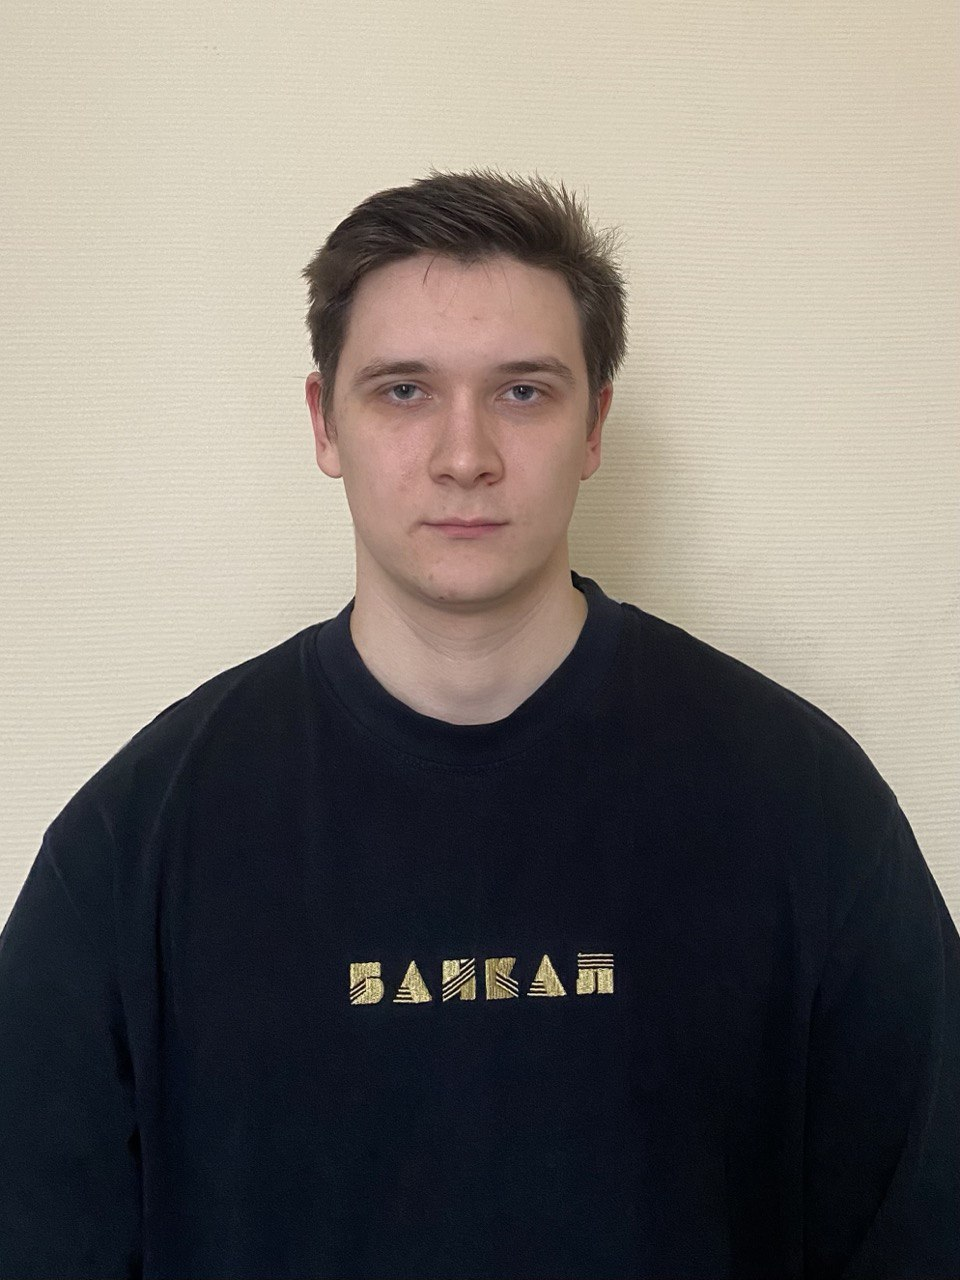
\includegraphics[height=3.7cm]{images/My_photo.jpg}}  \\
 && \\
 Студент 4 курса ФРКТ МФТИ &   & \\
 Кафедры ИСС&   & \\
 \\
Техник, лаб. 69 &\\ 
 \end{tabular}
\end{frame}
 
\section{\textbf{Проблема}}
\subsection{Введение}

\begin{frame}{Постановка Задачи}
\begin{figure}
    \centering
    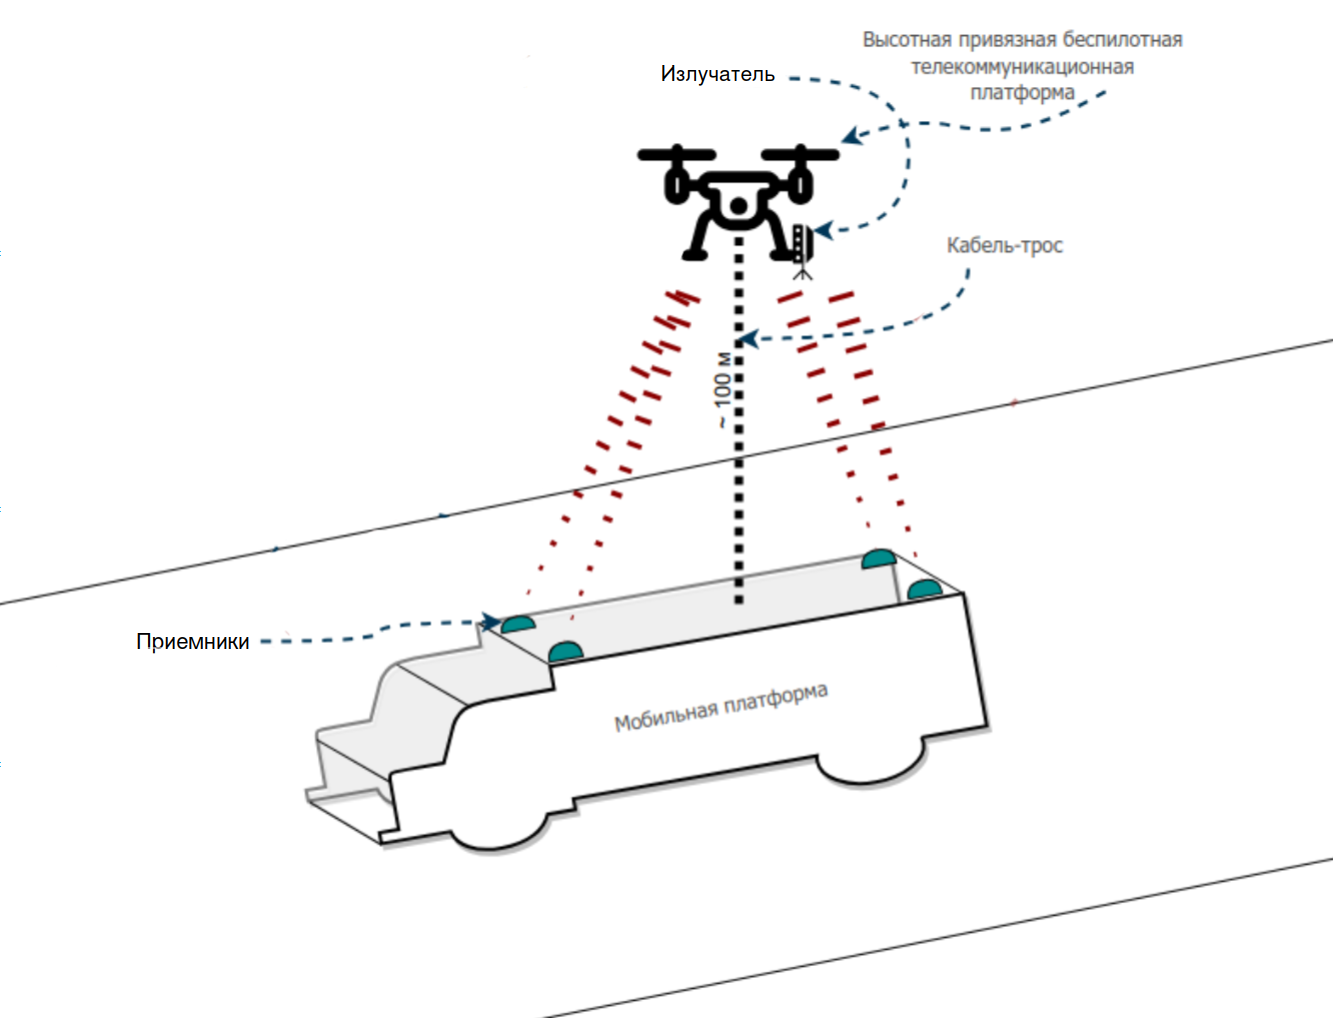
\includegraphics[width=0.7\linewidth]{images/system.png}
    \label{fig:placeholder}
\end{figure}


\end{frame}


\subsection{Формализация}
\begin{frame}{Задачи и цели исследования}

\begin{columns}
  \column{0.5\textwidth}
  \hspace*{1em}
  Цели исследования:
  \begin{itemize}
    \item Определить возможности системы:\\
    максимальная дальность, предельная точность
    
    \item Определить метод вычислений координат
    \item Разработать прототип ЛНС, провести испытания и собрать данные
  \end{itemize}

  \column{0.7\textwidth}
  \centering
  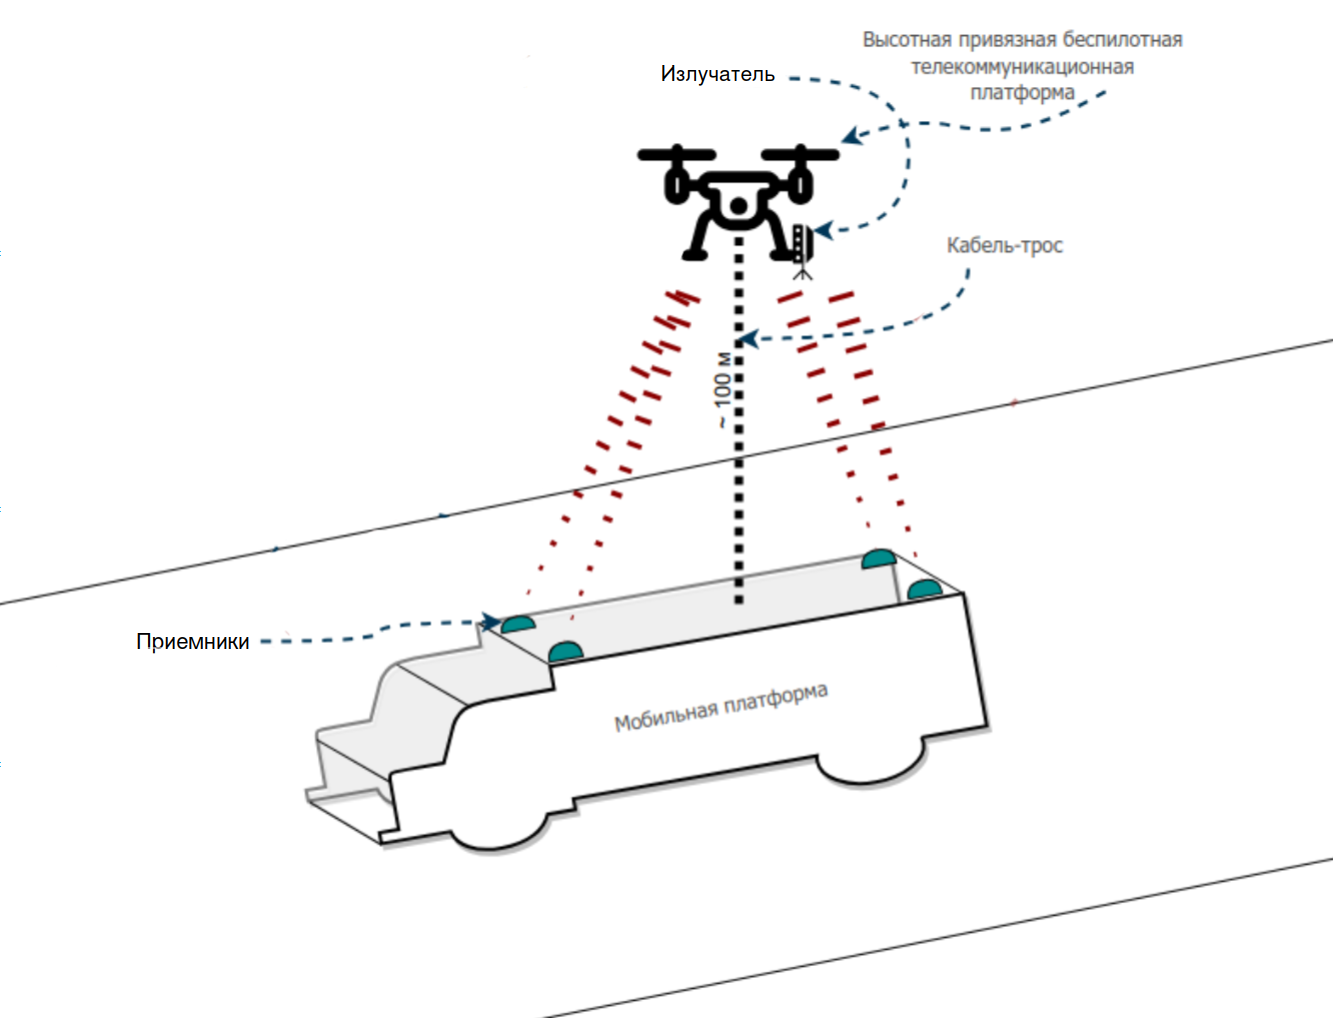
\includegraphics[width=\linewidth]{images/system.png}
\end{columns}
\end{frame}

\section{\textbf{Методология}}

\begin{frame}{Максимальная дальность}
I) Интенсивность звука в атмосфере затухает экспоненциально 
\begin{equation*}
I = I_0 e^{-\alpha r}, \text{ где}
\end{equation*}
{\footnotesize
\begin{align*}
\alpha &=
8.686 \, f^2
\Biggl[
\frac{1.84 \times 10^{-11}}{p}
\sqrt{\frac{T}{293.15}}
\\[0.5em]
&\quad+
\left(\frac{T}{293.15}\right)^{-5/2}
\left(
\frac{0.01275 e^{-2239.1/T}}{f_{r,\mathrm{O}} + f^2/f_{r,\mathrm{O}}}
+
\frac{0.1068 e^{-3352/T}}{f_{r,\mathrm{N}} + f^2/f_{r,\mathrm{N}}}
\right)
\Biggr],\text{ где}
\end{align*}
}
{\footnotesize
\begin{itemize}
\item $r$ - расстояние, м;
\item $f$ — частота звука, Гц;
\item $T$ — абсолютная температура, К;
\item $p$ — атмосферное давление, кПа;
\item $f_{r,\mathrm{O}}$, $f_{r,\mathrm{N}}$ — частоты релаксации кислорода и азота.
\end{itemize}
}

\end{frame}

\begin{frame}{Разделение ошибки}
    Разделим ошибку на состовляющие: Систематическую и случайную.
    \begin{figure}
        \centering
        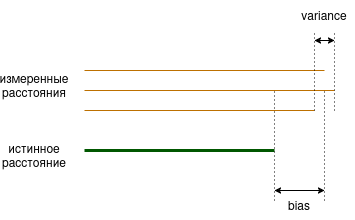
\includegraphics[width=0.8\linewidth]{./images/bias-variance.png}
    \end{figure}
    \end{frame}

\begin{frame}{Точность измерений}
Точность измерений расстояния зависит от разрешения часов приемников и излучателя:
\begin{equation}
 \pm d = \frac{c}{2 \Delta t}
\end{equation}

Приведем характерные значения:

\begin{table}[h!]
    \centering
    \begin{tabular}{|c|c|}
        \hline
        $\Delta t$ & $d$ \\
        \hline
        1 мкс & 0.17 мм  \\
        10 мкс & 1.7 мм \\
        100 мкс & 17 мм \\
        1000 мкс & 17 см \\
        \hline
    \end{tabular}
    \label{tab:example}
\end{table}
\end{frame}

\begin{frame}{Скорость звука}
Скорость звука в воздухе рассчитывается по формуле:
\begin{equation*}
\label{eq:speed-of-sound}
c = \sqrt{\gamma\,R_{\mathrm{mix}}\,T},
\end{equation*}
\vspace{0.3em}
где:
\begin{itemize}
  \item $c$ — скорость звука, м/с
  \item $\gamma = c_{p,\mathrm{mix}}/c_{v,\mathrm{mix}}$ — показатель адиабаты
  \item $R_{\mathrm{mix}} = R/M_{\mathrm{mix}}$ — удельная газовая постоянная смеси
  \item $T$ — абсолютная температура, К
  \item $M_{\mathrm{mix}} = (1-x_v)M_d + x_vM_v$ — молярная масса смеси
  \item $x_v = p_v/p$ — мольная доля водяного пара
  \item $p_v = h\,p_{\mathrm{sat}}(T)$ — парциальное давление водяного пара
\end{itemize}
\end{frame}

\begin{frame}{Погрешность скорости звука}
Полная погрешность:
\begin{equation*}
\Delta c = \sqrt{\left(\frac{\partial c}{\partial T}\Delta T\right)^2 + \left(\frac{\partial c}{\partial p}\Delta p\right)^2 + \left(\frac{\partial c}{\partial h}\Delta h\right)^2 + \Delta_{\text{мод}}^2}
\end{equation*}
\vspace{0.3em}
При типичных датчиках:
\begin{itemize}
  \item $\Delta T = \pm0.5\ ^\circ\mathrm{C}$ → $\Delta c_T \approx 0.30$ м/с
  \item $\Delta p = \pm120$ Па → $\Delta c_p \approx 0.06$ м/с
  \item $\Delta h = \pm3\%$ → $\Delta c_h \approx 0.002$ м/с
  \item $\Delta_{\text{мод}} \approx 0.31$ м/с
\end{itemize}
\vspace{0.3em}
\textbf{Результат:} $\Delta c \approx 0.43$ м/с ($\pm0.13\%$)
\end{frame}

\begin{frame}{Ошибка координат}
\textbf{GDOP (Geometric Dilution of Precision)} — коэффициент геометрического ослабления точности.
\vspace{0.3em}
\begin{columns}
  \column{0.5\textwidth}
  \hspace*{1em}
В силу относительно небольшого расстояния между приемниками на платформе, ошибка в плоскости XY будет значительной.\\
  \column{0.4\textwidth}
  \centering
  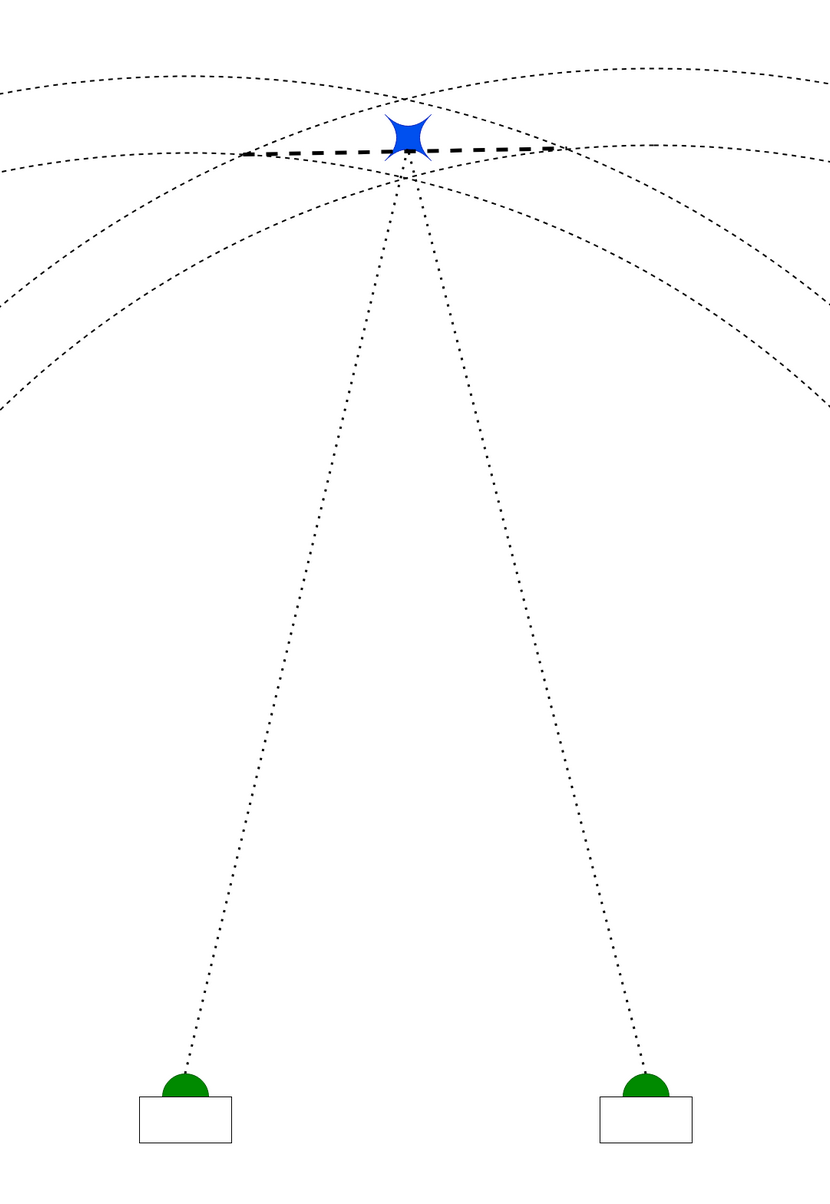
\includegraphics[width=\linewidth]{images/trilateration-geometry.png}
\end{columns}
\end{frame}

\begin{frame}{GDOP — формула}
\textbf{Модель: 4 якоря в вершинах квадрата со стороной $a$, объект на высоте $H$.}
\begin{equation*}
D = \sqrt{\frac{a^2}{2} + H^2} \quad \text{— расстояние до якоря}
\end{equation*}
\begin{block}{}
\centering
\boxed{\sigma_{xyz} = \sigma_d \cdot D \cdot \sqrt{\frac{2}{a^2} + \frac{1}{4H^2}}}
\end{block}
\vspace{0.3em}
где:
\begin{itemize}
  \item $\sigma_{xyz}$ — СКО положения в 3D
  \item $\sigma_d$ — ошибка измерения расстояния
  \item $a$ — сторона квадрата якорей
  \item $H$ — высота объекта
\end{itemize}
\end{frame}

\begin{frame}{GDOP — зависимость от геометрии якорей}
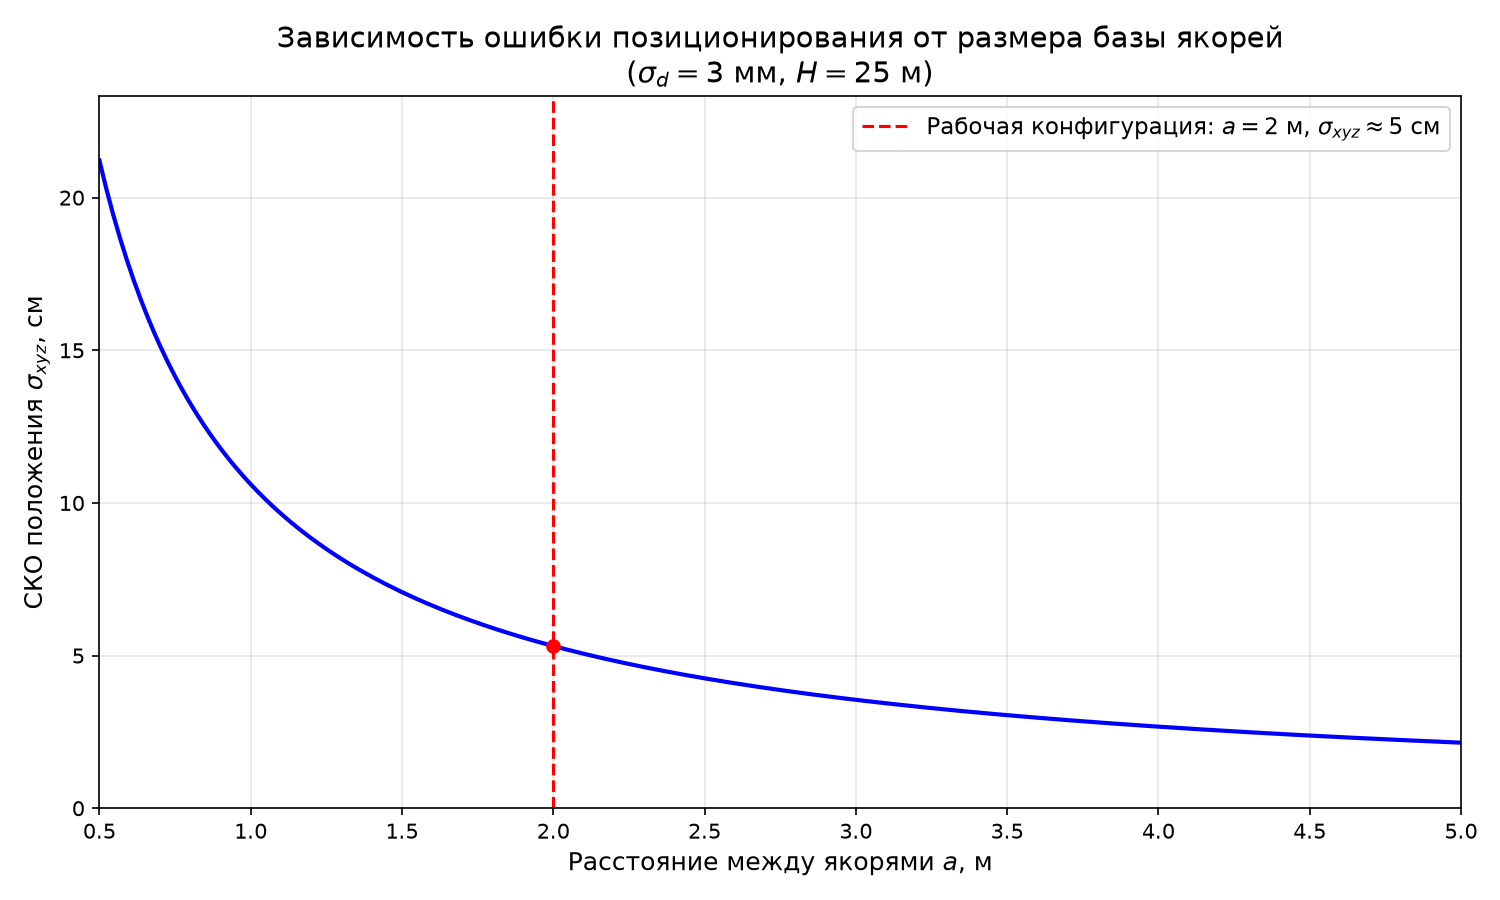
\includegraphics[width=\linewidth]{images/gdop-vs-anchor-distance.png}
\end{frame}

\begin{frame}{Вычислительный метод}
Метод Гаусса-Ньютона
\[
\boxed{%
\; \min_{\mathbf{p}}\; J(\mathbf{p}), \qquad
J(\mathbf{p}) = \sum_{i=1}^{N} w_i\bigl(\,\hat r_i - \|\mathbf{p}-\mathbf{a}_i\|\,\bigr)^2
}
\]

\begin{itemize}
  \item $\hat r_i$ \;— измеренное расстояние от якоря $i$ до объекта .
  \item $\mathbf{a}_i$ \;— вектор координат $i$-го якоря.
  \item $\mathbf{p}$ \;— вектор неизвестных координат объекта.
  \item $w_i$ \;— вес измерения $i$ (обычно обратный дисперсии).
  \item $J(\mathbf{p})$ \;— целевая функция суммы взвешенных квадратов невязок.
\end{itemize}
\end{frame}

\begin{frame}{Аналитический метод}
Координаты точки \(P\) удовлетворяют системе уравнений трёх сфер:
\[
(x - x_i)^2 + (y - y_i)^2 + z^2 = r_i^2, \qquad i = 1,2,3.
\]
\begin{align*}
2(x_2-x_1)x + 2(y_2-y_1)y &= r_1^2 - r_2^2 + x_2^2 - x_1^2 + y_2^2 - y_1^2, \\
2(x_3-x_1)x + 2(y_3-y_1)y &= r_1^2 - r_3^2 + x_3^2 - x_1^2 + y_3^2 - y_1^2.
\end{align*}

В матричной форме:
\[
A
\begin{pmatrix} x \\ y \end{pmatrix}
=
\begin{pmatrix} b_1 \\ b_2 \end{pmatrix},\begin{pmatrix} x \\ y \end{pmatrix} = A^{-1} \begin{pmatrix} b_1 \\ b_2 \end{pmatrix}.
\]

\[
z^2 = r_1^2 - (x - x_1)^2 - (y - y_1)^2,
z = \pm\sqrt{\,r_1^2 - (x - x_1)^2 - (y - y_1)^2\,}.
\]
\end{frame}

\begin{frame}{Аналитический метод}

  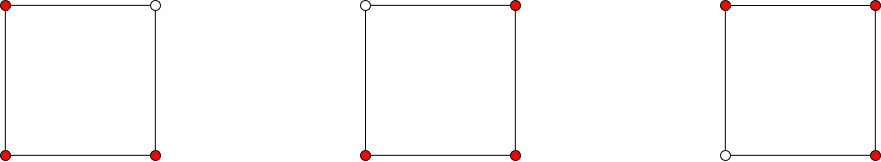
\includegraphics[width=\linewidth]{images/anchor-triplet-selection.png}

\end{frame}

\begin{frame}{Сравнение}
Зависимость ошибки локализации от дисперсии шума измерений.
\begin{figure}
    \centering
    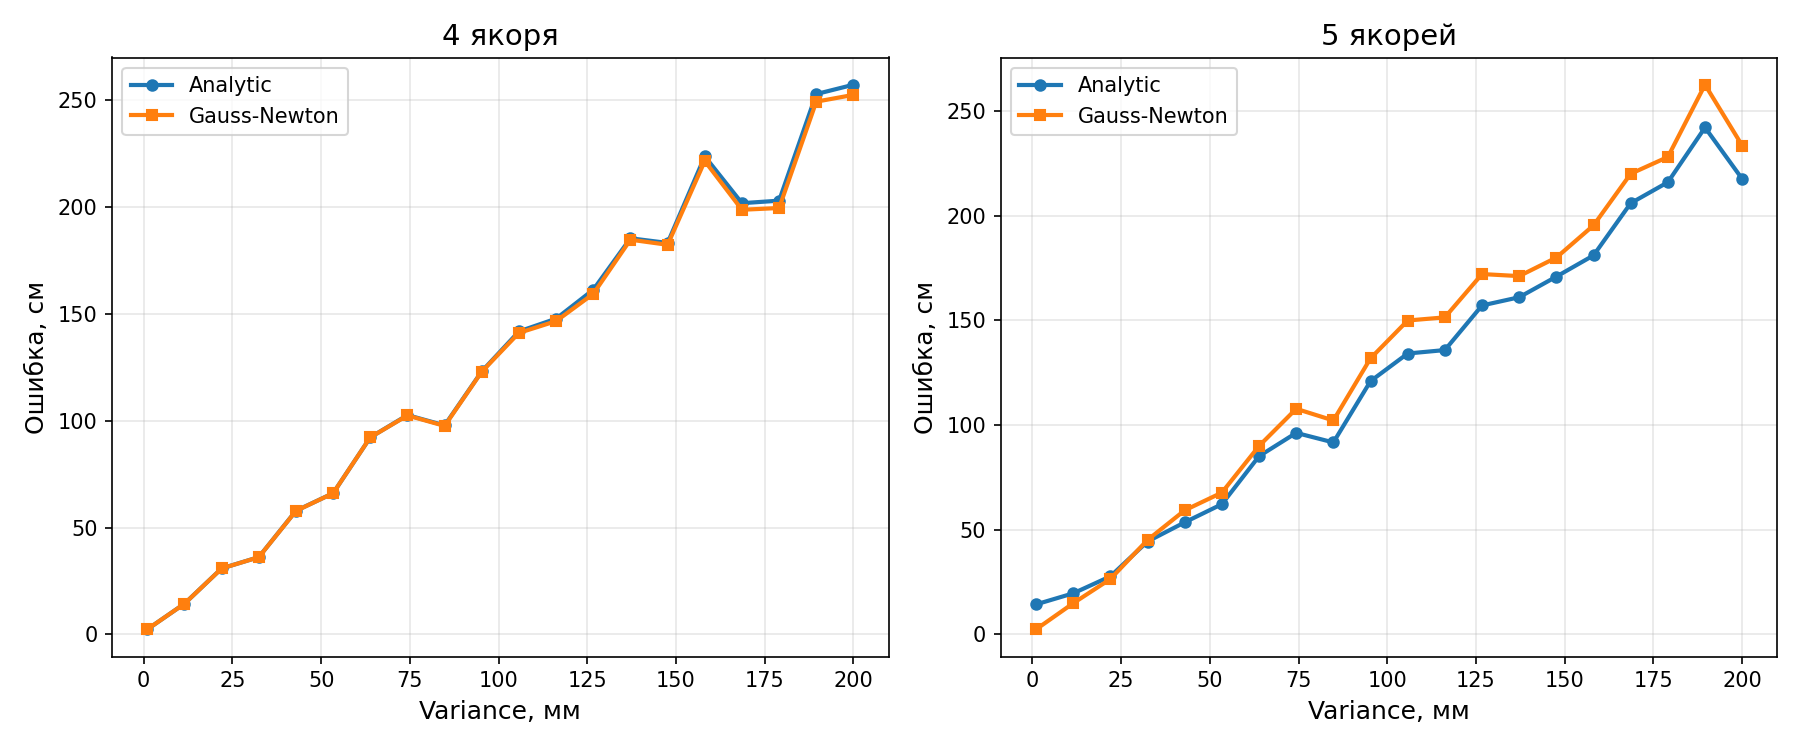
\includegraphics[width=1\linewidth]{./images/error_vs_variance.png}
\end{figure}

\end{frame}

\begin{frame}{Таблица погрешности}
\begin{table}[h!]
    \centering
    \caption{Аналитический метод, $H=20$м}
    \begin{tabular}{|c|c|c|}
        \hline
        $\sigma$, м & 4 якоря, см & 5 якорей, см \\
        \hline
        0.002 & 3.56 & 16.00 \\
        \hline
        0.005 & 6.79 & 17.27 \\
        \hline
        0.01 & 12.12 & 18.18 \\
        \hline
        0.05 & 56.46 & 64.39 \\
        \hline
        0.1 & 132.64 & 110.75 \\
        \hline
    \end{tabular}
\end{table}
\begin{table}[h!]
    \centering
    \caption{Метод Гаусса-Ньютона, $H=20$м}
    \begin{tabular}{|c|c|c|}
        \hline
        $\sigma$, м & 4 якоря, см & 5 якорей, см \\
        \hline
        0.002 & 3.59 & 3.67 \\
        \hline
        0.005 & 6.33 & 6.60 \\
        \hline
        0.01 & 14.69 & 11.91 \\
        \hline
        0.05 & 67.07 & 65.10 \\
        \hline
        0.1 & 122.23 & 122.88 \\
        \hline
    \end{tabular}
\end{table}
\end{frame}


\section{\textbf{Вопросы}}
    
\begin{frame}
\centering 
{\bf Спасибо за внимание!}
\end{frame}

\end{document}